% ------ PREAMBLE ------ 
\documentclass[11pt,a4paper]{article}
\usepackage[scaled=0.85]{FiraMono}
\usepackage[utf8]{inputenc}
\usepackage[english]{babel}
\usepackage[margin=2cm]{geometry}
\renewcommand{\baselinestretch}{1.5} 
\usepackage{indentfirst}
% ------ font ----------
\usepackage{sansmathfonts}
\usepackage{fontspec}
\setmainfont{Latin Modern Sans}
% ------ math ----------
\usepackage{physics}
\usepackage{algpseudocode}
\AtBeginDocument{\RenewCommandCopy\qty\SI}
\usepackage{amsmath,amsfonts,amssymb}
\newcommand\inlineeqno{\stepcounter{equation}\ 
\usepackage{derivative}
\DeclareDifferential{\dd}{\mathrm{d}}
\usepackage[shortlabels]{enumitem}
\usepackage{siunitx}
\sisetup{detect-all,
	separate-uncertainty = true,
	uncertainty-separator = {\,\pm\,},
	multi-part-units=single
}
\DeclareSIUnit{\year}{yr}

% ---- graphics ----
\usepackage{graphicx}
\graphicspath{{../figures/}}
\usepackage{subfig}
\usepackage{float}
\usepackage{caption}
\captionsetup{font={small, color={Gray2}}, labelfont={sf, bf}, textfont={sf,sansmath}, labelsep=colon}
\usepackage[dvipsnames]{xcolor}
\definecolor{Gray1}{RGB}{101, 101, 101}
\definecolor{Gray2}{RGB}{60, 60, 60}
\definecolor{Code}{RGB}{230, 235, 255}
\usepackage[most]{tcolorbox}
\tcbset{on line, 
	boxsep=4pt, left=0pt,right=0pt,top=0pt,bottom=0pt,
	colframe=white,colback=Code,  
	highlight math style={enhanced}
}
\let\oldtexttt\texttt
\renewcommand{\texttt}[1]{\tcbox[boxsep=1pt, left=2pt, right=2pt]{\oldtexttt{#1}}}
\usepackage[colorlinks=true, 
linkcolor=Plum, 
citecolor=RoyalBlue, 
urlcolor=BlueViolet]{hyperref}
% --- text formatting ---
\usepackage{booktabs}
\usepackage{multirow}
\usepackage{setspace}
\usepackage{pdfpages}
\usepackage{pythonhighlight}
\usepackage{verbatim}
\usepackage{fancyhdr}
\usepackage{lipsum}
\pagestyle{fancy}
\fancyhf{} 
\fancyhead[L]{\leftmark}
\fancyfoot[C]{\thepage}
\usepackage{setspace}\onehalfspacing
\AtBeginDocument{%
	\addtolength\abovedisplayskip{-0.5\baselineskip}%
	\addtolength\belowdisplayskip{-0.5\baselineskip}%
	%  \addtolength\abovedisplayshortskip{-0.5\baselineskip}%
	%  \addtolength\belowdisplayshortskip{-0.5\baselineskip}%
}
% --- formatting titles according to parts ---
\usepackage{titlesec}
\usepackage{etoolbox}
\definecolor{part1color}{RGB}{31, 78, 121}    % Dark Blue (Intro)
\definecolor{part2color}{RGB}{200, 110, 10}   % Dark Orange (Material)
\definecolor{part3color}{RGB}{46, 125, 50}    % Dark Green (Methods)
\definecolor{part4color}{RGB}{197, 27, 125}   % Dark Red (Results)
\definecolor{part5color}{RGB}{125, 73, 198}   % Dark Purple (Discussion)
\newcommand{\setpartcolor}[1]{%
	\titleformat{\part}
	{\color{#1}\titlerule[1pt]\LARGE\fontseries{sbc}\sffamily\selectfont\color{#1}}
	{\thepart}
	{0.5em}
	{}
	[\vspace{-0.8em}]
	\titleformat{\section}
	{\Large\fontseries{sbc}\sffamily\selectfont\color{#1}}
	{\thesection}
	{0.6em}
	{}
	[\vspace{-0.5em}]
	\titleformat{\subsection}
	{\large\fontseries{sbc}\sffamily\selectfont\color{#1}}
	{\thesubsection}
	{0.4em}
	{}
	[\vspace{-0.5em}]
	\titleformat{\subsubsection}
	{\normalfont\fontseries{sbc}\slshape\sffamily\color{#1}}
	{\thesubsection.\alph{subsubsection}}
	{0.4em}
	{}
	[\vspace{-0.5em}]
	\titleformat{\paragraph}
	{\normalfont\fontseries{sc}\fontshape{sl}\sffamily\color{#1}}
	{\theparagraph}
	{0.4em}
	{\vspace{-0.8em}}
	[\vspace{-0.8em}]
}
% --- shortcuts commands ---
\newcommand{\ie}{\emph{i.e.}, }
\newcommand{\eg}{\emph{e.g.}, }
\newcommand{\ssaunit}{\meter\squared\per\kilo\gram}
\newcommand{\ssa}{\mathrm{SSA}}
\newcommand{\sza}{\mathrm{SZA}}
\newcommand{\lwdn}{\mathrm{LW}^{\downarrow}}
\newcommand{\mycaption}[2]{\caption{\textbf{#1} | #2}}

\usepackage[backend=biber, style=apa]{biblatex}
\addbibresource{Stage_IGE_2026.bib}

% ////////////////////////////////////
% ///////////// DOCUMENT ///////////// 
% ////////////////////////////////////

\begin{document}
	\title{Internship report}
	
	\tableofcontents
	\newpage

\setpartcolor{part1color}
\part{Introduction}
Snow is one of the major component of the cryosphere. Its global distribution on both ocean and land areas strongly depends on seasonality, latitude, and elevation. It occurs in three forms, mainly: permanent snow on ice sheets and glaciers, snow on sea ice, and seasonal snow cover. The latter is estimated to account for 1.3\% (summer) to 30.6\% (winter) of the Northern Hemisphere land surface \parencite{Vaughan2013}, with the 1967-2026 mean snow cover extent (SCE hereafter) in winter being around \qty{39.79e6}{\kilo\meter\squared} \parencite{rutgers_snowlab}. Sea ice is almost completely covered by snow during the winter season; its peak concentration, therefore representative of sea ice specific SCE, occurs in March in the Northern Hemisphere (\qty{15.03e6}{\kilo\meter\squared}) and in September in the Southern Hemisphere (\qty{18.61e6}{\kilo\meter\squared}) \parencite{warrenSnowDepthArctic1999, fettererSeaIceIndex2025}. Finally, perennial snow mean extent over the 2000-2022 period is estimated at \qty{16.47e6}{\kilo\meter\squared} from NASA's Moderate Resolution Imaging Spectroradiometer (MODIS), including glaciers, ice caps, Greenland and Antarctica ice sheets \parencite{johnstonGlobalSnowSeasonality2024}.\\
These several tens of millions of snow-covered squared kilometres play a major role in freshwater resources availability, ecosystems equilibrium and, particularly, climate regulation. In fact, among its many physico-chemical properties, snow represents one of the strongest reflective materials on Earth's surface. The fraction of solar radiation delivered to a body that is diffusely reflected by it is called \emph{albedo}; for snow, this amount is roughly close to 1, since its highest reflectivity occurs in the range of visible light, \ie where solar radiation intensity peaks \parencite{kokhanovskyScatteringOpticsSnow2004}. Thanks to its high albedo, snow represents of the main contributors to Earth's energy budget regulators \parencite{NSIDC_cryosphere}. Of the \qty{340}{\watt\per\meter\squared} of net solar radiation incident at the top of the atmosphere, Northern Hemisphere land snow cover alone reflects approximately \qty{2}{\watt\per\meter\squared} back to space, averaged over the 1979--2008 period; in May, when SCE and soil insulation are highest, this quantity can reach \qty{4.5}{\watt\per\meter\squared} \parencite{flannerRadiativeForcingAlbedo2011}. Without the year-average radiative forcing from land snow cover alone, Earth's surface temperature would be approximately \qty{0.54}{\kelvin} higher than the current planetary mean. This estimate follows from linearising the Stefan-Boltzmann law with respect to temperature, assuming that Earth radiates as a blackbody with no feedback effects, making it a lower-bound estimate. In fact, real climate feedbacks (water vapour, lapse rate, clouds) reduce the effective restoring force, amplifying the true temperature response \parencite{croninHowWellWe2023}.\\
As the whole cryosphere in general, snow distribution on Earth is undergoing dramatic changes because of the current anthropogenic perturbation of the climate system and warming of the atmosphere. At the global scale, SCE is experiencing a negative trend since the 1980s, with a statistically significant reduction in the mean area of 5\% after 1988, compared to the 1967-1988 period, in the Northern Hemisphere only, and an earlier melt onset in the spring season \parencite{robinsonSeasonalVariabilityNorthern2000, dyeVariabilityTrendsAnnual2002}. Less snow cover in both space and time, driven by rising temperatures, reduces terrestrial albedo and increases the absorption of incoming solar radiation at the surface, which in turn amplifies warming \parencite{cubaschProjectionsFutureClimate2001, hollandPolarAmplificationClimate2003}. This mechanism is known as the positive snow--
albedo feedback: it is estimated to be responsible of a reduction in Northern Hemisphere land snow cover radiative cooling forcing of $\sim\qty{0.22}{\watt\per\meter\squared}$ from 1979 to 2007, which nearly equals the contribution of Arctic sea ice \parencite{flannerRadiativeForcingAlbedo2011}. The magnitude of such feedback is further amplified when light-absorbing particles, such as dust, black carbon and microbial growth, deposit on the surface of snowpack \parencite{skilesLightAbsorbingParticles2018}. 
	
It is clear, at this point, that developing a proper understanding of how snow interacts with solar radiation is crucial for a better understanding of the evolution of the climate system. Snow optical properties, particularly albedo, are directly related to density and grain type, and are strongly wavelength-dependent \parencite{kokhanovskyScatteringOpticsSnow2004, bohrenTheoryOpticalProperties1974}. Quantifying these properties involves radiative transfer calculations extended to the uppermost part of the snowpack, which must be assumed to be composed of individual grains of a given size and shape. Many studies have adopted equivalent spheres, assuming they can properly represent any other shape at a given optical diameter \parencite{bohrenTheoryOpticalProperties1974, warrenSnowDepthArctic1999}. However, recent studies demonstrated that this approach is not satisfactory when it comes to specific properties such as the single-scattering albedo -- the fraction of intercepted radiation that is scattered rather than absorbed -- and the bidirectional reflectance distribution function (BRDF) -- the reflectance of a surface for a specific combination of illumination and viewing directions \parencite{kokhanovskyScatteringOpticsSnow2004, liboisInfluenceGrainShape2013, dumontHighaccuracyMeasurementsSnow2010}. For this reason, when addressing grain size, a more general, shape-independent quantity is preferable to the optical diameter: the \emph{specific surface area} (SSA), defined as the total surface area of snow grains per unit mass -- expressed in \unit{\meter\squared\per\kilo\gram} \parencite{internationalunionofpureandappliedchemistryiupacSpecificSurfaceArea}. This quantity, used hereafter to address snow grain size, largely influences snow reflectance for wavelengths in the Near-Infrared (NIR) range, between \qty{750}{\nano\meter} and \qty{1400}{\nano\meter} particularly \parencite{warrenModelSpectralAlbedo1980}. For example, a factor-6 decrease in the SSA (\eg from 60 to \qty{10}{\ssaunit}) can approximately reduce albedo of ~15\% at \qty{1000}{\nm}. In general, albedo decreases monotonically with SSA and can be modelled as an exponential function of $\ssa^{-1/2}$ \parencite{kokhanovskyScatteringOpticsSnow2004}.
	
Snow grain size dynamics are therefore a key indicator of how snowpack optical properties evolve over time and space, making their tracking essential. Changes in grain size are primarily driven by processes such as metamorphism, wind drift, and precipitation.\\
When transformations in size and shape occur below the melting point ($T = \qty{0}{\celsius}$), the metamorphism is dry: the grain size grows at a rate defined by the respective increase in temperature and temperature gradient \parencite{colbeckOverviewSeasonalSnow1982}. Instead, if snow is at the melting point, the liquid water content directly drives the size increase, which is faster than in the the dry case -- we talk about wet metamorphism, in this case \parencite{wakahamaMetamorphismWetSnow1968}. Anyway, independently of the type of metamorphism, the change in size is always positive and irreversible \parencite{find a cit}.\\	
Transportation by the wind occurs when its velocity breaks snow cohesion and lifts grains. This is more likely for fresh-fallen snow than for old, metamorphosed snow \parencite{lenaertsMeltwaterProducedWind2017}. This process, called wind drift, varies with wind speed: saltation occurs under weak winds, with snow skipping a few centimeters above the surface, while stronger winds create snow plumes, lifting grains up to hundreds of meters -- the so-called blowing snow \parencite{adokSnowDrift1977, WMO2024BlowingSnow}.
Wind drift has two opposing effects on grain size. Erosion of the snowpack’s upper layers exposes older, coarser, and less reflective layers \parencite{lenaertsMeltwaterProducedWind2017}. Conversely, wind fractures grains through collisions, so newly formed deposits typically consist of finer grains \parencite{domineThreeExamplesWhere2009}.\\
Snow fall is generally responsible of depositing fresh and more fine-grained snow at surface, potentially covering already metamorphosed and coarser layers, thus increasing SSA an albedo \parencite{domineThreeExamplesWhere2009}.
	
This study is focused on the temporal evolution of snow and its albedo over the whole Antarctica, where all the processes of above act and interplay in a complex manner, over a wide range of climatic and geographical contexts. The Antarctic Ice Sheet (AIS), expanding for \qty{14e6}{\kilo\meter\squared} over 98\% of the continent, is almost completely snow-covered year-round. As a polar region, it plays a massive role in positive climate feedback. At the same time, compared to the Arctic, Antarctica presents unique challenges for the exploration of surface radiative properties.\\
Being such a harsh and inaccessible place, it has only allowed \emph{in situ} investigations limited to regional scales and relatively short time coverage. This has led the scientific community to rely on satellite data, which inherits higher uncertainties and reduced spatio-temporal resolution, from missions such as AVHRR, MODIS, and CLARA-A2.1-SAL \parencite{callejaSnowAlbedoSeasonality2019, sunChangesAntarcticsSummer2023}.\\
Moreover, many of the AIS surface processes are not yet properly understood, particularly toward the center of the ice sheet. One of these is the mechanism involved in the formation of snow megadunes. These are antidune-like sedimentary forms, whose fields cover a large fraction of the central part of the AIS (\qty{500e5}{\kilo\meter\squared}) \parencite{frezzottiSnowMegadunesAntarctica2002}. They have relatively small amplitudes (1--\qty{8}{\meter}), compared to their wavelength (2--\qty{4}{\kilo\meter}), and crest lengths of 10 to \qty{100}{\kilo\meter} \parencite{fahnestockSnowMegaduneFields2000}---these characteristics prevented their observation until the beginning of satellite exploration over the continent. Their formation likely results from a complex interplay between geomorphological and meteorological conditions that causes a cryosphere-atmosphere feedback mechanism: katabatic winds, blowing toward the outer boundaries of the AIS from the center, affect local topography by deposition-erosion processes. Topography, in turn, modifies the katabatic wind field; megadunes develop perpendicularly to the main direction of such winds \parencite{}. Still, the way snow grain size evolves on these structures remains an unexplored topic.\\
With this work, we aim to improve the understanding of surface albedo evolution in Antarctica by combining \emph{in situ} measurements with satellite observations. Using data from automated albedometers installed at several locations on the AIS, we will produce time series of locally measured specific surface area (SSA) and compare them with satellite-retrieved grain size. Measurement stations were deployed in two primary locations: on the coast near the French station Dumont d'Urville, and in a megadune field, with one albedometer on the erosion area and another on the accumulation area of a dune.

The overarching goals of this analysis are:
\begin{itemize}[noitemsep]
	\item to validate a satellite product, ESA's Sentinel-3 Ocean and Land Color Instrument, enabling long-term and continent-wide studies of snow albedo at a relatively fine resolution ($\sim\qty{300}{\meter}$), compared to other missions (e.g., MODIS);
	\item to deepen the understanding of processes driving temporal albedo changes at the local scale, particularly on megadunes, using an unprecedented 6-year continuous \emph{in situ} record of snow albedo.
\end{itemize}

The analysis is structured as follows:
\begin{enumerate}[noitemsep]
	\item \textbf{Processing of \emph{in situ} data}: upgrading and optimizing the existing workflow developed by \cite{arioliDynamicsSnowGrain2023}; this includes both processing data from the main instrument (Multiband and relative weather stations) and from Solalb, a second albedometer used as as external reference to asses the quality of Multiband and Sentinel-3 performaces;
	\item \textbf{Processing of Sentinel-3 data}: downloading the frames and executing the SICE 1.6 algorithm, as described by \cite{kokhanovskyRetrievalSnowProperties2019};
	\item \textbf{Comparison of the time series}: performing corrections to address possible gaps between the two datasets and interpreting the retrieved albedo dynamics geoscientifically.
\end{enumerate}

\setpartcolor{part2color}
\part{Material and methods}

	\section{Theoretical backgrounds}
	
	!!! This risks to become "textbook"-like - then, must be SUPER ADAPTED TO MY SPECIFIC GOAL AND BE VERY PERSONAL AND NOT GENERAL AT ALL - PASSIONATING !
	write it after matmethods and results
	
	\section{Study area: an overview of the station}
	
	\section{Material and instruments}
	
		\subsection{\emph{In situ}: the Multiband albedometer}
\begin{figure}
	\centering
	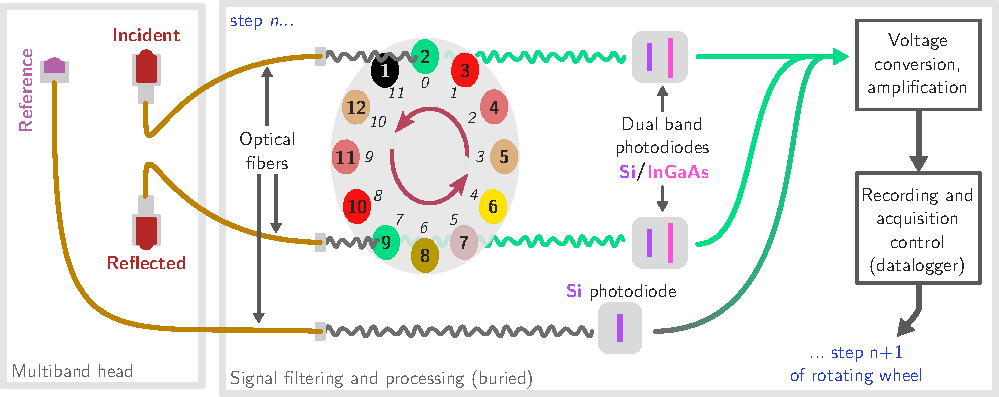
\includegraphics[width=16cm]{mbscheme.pdf}
	\mycaption{Structure of Multiband}{Long caption}
	\label{fig:mbscheme}
\end{figure}
The main instrument used in this study is the Multiband albedometer, developed at Grenoble’s Institute for Geosciences of the Environment (IGE) and fully described in \cite{arioliDynamicsSnowGrain2023}. It is a robust automated optical radiometer capable of acquiring solar radiation across a discrete set of bands, from the visible to the short-wave infrared, which are essential for retrieving snow surface albedo.
Similar to previously developed albedometers (e.g., Autosolexs, Solalb; see \cite{picardDevelopmentCalibrationAutomatic2016a}), the Multiband consists of a set of metal gantries. One perfectly leveled pole projects the instrument head horizontally at $\sim\qty{3}{\meter}$ from the installation point and at a height of $\sim\qty{2}{\meter}$ above the snow surface, typically oriented north- or southward to minimize shadowing from other components. The head features two custom cosine-shaped light collectors, one pointing upward and the other downward, to measure incident and reflected irradiance, respectively. These collectors, meticulously designed by \cite{picardDevelopmentCalibrationAutomatic2016a}, incorporate a bumped Teflon surface to maximize performance at any solar zenith angle (SZA), including grazing angles, which are critical for accurate radiation measurements.

The signal is transmitted to the instrument’s recording unit via two Ocean Optics QP800-VIS-NIR optical fibers, each $\qty{6}{\meter}$ long with a $\qty{800}{\micro\meter}$ core diameter. Unlike earlier albedometers, where optical fibers directly sent the signal to a spectrometer for high-resolution ($\qty{3}{\nano\meter}$) spectral recording, the Multiband employs a more energy-efficient approach. The broadband radiation transmitted by the fibers passes through a set of polarizing filters mounted on a $\sim\qty{20}{\centi\meter}$ wheel with 12 slots. These filters are Edmund Optics’ TECHSPEC® hard-coated optical density (OD) 4.0, $\qty{25}{\nano\meter}$ bandpass filters, specific for wavelengths of 500, 600, 800, 925, 1050, 1300, and \qty{1550}{\nano\meter}. During a full measurement cycle ($\qty{30}{\second}$), the wheel rotates to acquire spectral measurements for each selected wavelength from both the incident and reflected signals. These signals are transmitted to dual-band Silicon (Si) / Indium-Arsenide-Gallium (InGaAs) photodiodes (DSD2, Thorlabs). Measurements on the two channels are simultaneous, and the wheel includes duplicate filters to ensure synchronous recordings at the most relevant wavelengths, as well as one capped slot to measure the dark current (\ie background thermal noise) -- see Figure \ref{fig:mbscheme} for details.
The signals registered by the dual photodiodes are amplified by a high-gain electronic board. Finally, a Campbell Scientific CR1000x data logger records the spectral radiation in \unit{\milli\volt}. Since the duration of a full measurement cycle is long enough for atmospheric conditions to potentially change, a measure of ambient light is also recorded at every step: a third upward-facing optical fiber transmits incoming radiation to a Si photodiode (FDS100, Thorlabs). This photodiode acquires a wideband measurement in the 350--\qty{1100}{\nano\meter} range, referred to as the reference, expressed in light counts. Its signal undergoes the same voltage amplification and recording steps as the spectral measurements; for a single cycle, 12 references are registered.

The entire system’s electronics are powered by a solar panel. The Multiband has demonstrated its durability by acquiring continuous measurements without interruption at each of the stations where it was installed.

		\subsection{\emph{In situ}: the Solalb albedometer}
		
		\subsection{\emph{In situ}: automatic weather stations (AWS)}
	
		\subsection{Satellite imagery: Sentinel-3 Ocean Land and Colour Instrument}
		
			\subsubsection{Generalities}
			
Orbit, resolution, swath, revisit time etc.

			\subsubsection{Data availability}
			
	
	\section{Methods}
	
		\subsection{Processing of Multiband data}
		
\begin{figure}
	\centering
	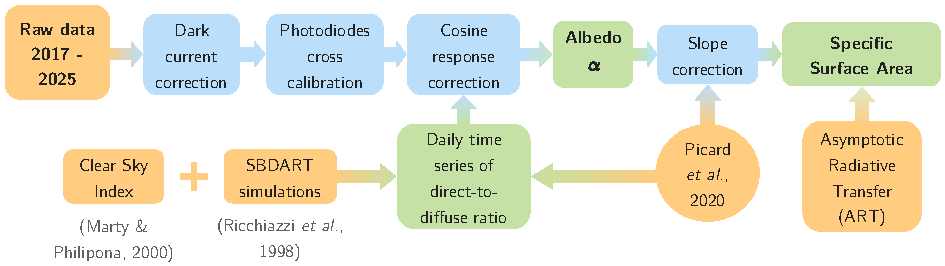
\includegraphics[width=16.5cm]{mbwf.pdf}
	\mycaption{Workflow of Multiband processing}{Modified after \cite{arioliDynamicsSnowGrain2023}}
	\label{fig:mbwf}
\end{figure}

			\subsubsection{Overview of the existing algorithm}
The pipeline for processing Multiband data is summarized in Figure~\ref{fig:mbwf} and builds on the work of \cite{arioliDynamicsSnowGrain2023}. It executes functions from a custom Python library specifically developed for this purpose (the \texttt{generic\_algorithm}), along with utilities from the open-source module \texttt{snowoptics} (\href{https://github.com/ghislainp/snowoptics}{GitHub}), a library for retrieving snow optical properties based on the Asymptotic Radiative Transfer theory (ART, \cite{kokhanovskyScatteringOpticsSnow2004}). This processing had already been applied to measurements acquired by all three Cap Prud'Homme stations (D5, D10, D17) until 2022 in \cite{arioliDynamicsSnowGrain2023}'s work.

\begin{enumerate}[align=right,itemindent=2em,labelsep=4pt,labelwidth=1em,leftmargin=0pt,nosep]
	\item \textbf{Raw data filtering}\\
A preprocessing step excludes low-quality data, including: (i) measurements acquired at $\sza > \ang{70}$ due to the limited performance of cosine collectors at low solar angles; \parencite{picardDevelopmentCalibrationAutomatic2016a}; (ii) measurements acquired under varying or low ambient light conditions, if the standard deviation of the 12 references recorded during a cycle exceeds 1\% of their mean radiance; and (iii) all records at \qty{1550}{\nano\meter} due to the poor signal-to-noise ratio.
	\item \textbf{Dark current}\\
The measurements are corrected for the background thermal noise of the photodiodes. Four dark currents are registered at every cycle (Si and InGaAs, for both the incident and reflected channels) and subsequently subtracted from the respective channel's spectral irradiance. For example, for the reflected channel, the dark corrected spectral signal $i_{\mathrm{dc}}^{\mathrm{ref}}(\lambda)$ results from:
\begin{equation}
	i_{\mathrm{dc}}^{\mathrm{ref}}(\lambda) = i^{\mathrm{ref}}(\lambda) - i_{\mathrm{dark}}^{\mathrm{ref}}(\lambda)
\end{equation}
	\item \textbf{Cross-calibration}\\
The incident and reflected signals passing through the cosine collectors and the optical fibers naturally differ due to varying transmissivity and sensitivity of the components in the two channels. To account for this, a parallel cross-calibration is performed during the installation of the albedometers. This involves orienting both light collectors upward and side-by-side to record the same irradiance over two days at an hourly resolution (every 10 minutes at solar noon). The two signals are then corrected following steps 1 and 2 of the current processing chain, averaged, and their ratio is multiplied by every incident spectrum measured during the operational stage of the albedometer to compensate for differences in the electronic response of the two channels. 
	\item \textbf{Cosine response correction}\\
Each light collector behaves uniquely at different solar angles under perfectly direct light conditions, with its response always diverging by a given amount from an ideal cosine curve. For this reason, before deployment in the field, every collector's response is calibrated in the lab by illuminating it with a direct light beam at different angles. This experimental response is used to normalize every measurement. Since this correction step only involves the direct component of the incident radiation -- not its diffuse part or the fully diffused reflected light -- the direct-to-diffuse light ratio must be quantified for every measurement. This ratio depends on: (i) atmospheric characteristics at the specific geographical location (longitude, latitude, altitude); (ii) solar elevation, \ie the SZA; and (iii) meteorology at the time of the measurement, particularly cloud cover. To account for the first two factors, a time-independent, direct-to-diffuse partitioning is simulated using the Santa Barbara DISORT Atmospheric Radiative Transfer (SBDART) model \parencite{ricchiazziSBDARTResearchTeaching1998}. Cloud cover is quantified using the 30-minute resolution recordings of the AWS located near the albedometers, with the methodology proposed by \cite{martyClearskyIndexSeparate2000}. These two steps will be detailed later.
	\item \textbf{Albedo calculation}\\
The ratio between the corrected incident and reflected records yields a first spectral albedo, $\alpha(\lambda)$, which, at this stage, is assumed to be for a plane and flat surface. Values of $\alpha < 0$ and $\alpha > 1.5$ are discarded.
	\item \textbf{Slope correction}\\
Albedo is then corrected for potential slope and surface irregularities (\eg sastrugi) characterizing the snow surface on the day of the measurement, following \cite{picardSpectralAlbedoMeasurements2020}. The custom function \texttt{generic\_algorithm.albedo\_timeseries\_correction} is used to iteratively compute the unknown slope parameters that best fit the within-day evolution of the previously retrieved albedo spectra. At the end of this step, a daily averaged, slope-corrected albedo spectrum is produced.
	\item \textbf{SSA estimate}\\	
\cite{kokhanovskyScatteringOpticsSnow2004}'s ART theory is finally used to compute the snow grain size (SSA) from the daily albedo, as previously described in the theoretical background section.
\end{enumerate}

			\subsubsection{New implementations}
We extend the pipeline to the latest 2026 records and to the two stations installed on a megadune during the 2019 EAIIST campaign. Additionally, we focus on characterizing the atmosphere at the two main locations and perform diagnostics to investigate potential instrumental issues.
			
				\paragraph{Direct-to-diffuse light ratio}
Simulations of direct/diffuse partitioning with SBDART consist of computing SZA-specific spectral irradiance curves, both of global and diffuse fraction, and taking their ratio. We performed these calculations for the megadunes area using the following model parameters: \texttt{pristine} atmosphere (likely no pollution in the centre of the AIS), \texttt{sub-arctic winter} atmosphere type (the closest option available), \qty{3000}{\meter} a.s.l. elevation, temperature $T = \qty{-35.8}{\celsius}$, relative humidity $\mathrm{RH} = 0.70$, with the last two parameters being the daily average in the megadunes area over the 2019--2026 summers, retrieved from the CNR4 records. The ratio is computed for wavelengths between \qty{0.3}{\micro\meter} and \qty{4}{\micro\meter} at a \qty{0.2}{\micro\meter} resolution.

				\paragraph{Clear Sky Index (CSI)}
\cite{martyClearskyIndexSeparate2000} proposed a technique to discriminate between overcast and clear-sky conditions using the \emph{Clear Sky Index} (CSI), which involves comparing the emissivity of the observed atmosphere with that of an ideal cloud-free atmosphere with the same properties. Clouds generally increase the emittance of the atmosphere, as they act as near-blackbodies in the thermal infrared. The emissivity of the atmosphere can be directly derived from air temperature $T_A$​ and the incoming long-wave radiation $\lwdn$ using the Stefan-Boltzmann law:
\begin{equation}
	\epsilon_{A} = \frac{\lwdn}{\sigma T_A} \qquad (-)
\end{equation}
with $\sigma = \sim\qty{5.67e-8}{\watt\meter^{-2}\kelvin^{-4}}$ being the Stefan-Boltzmann constant. To determine the apparent emissivity of a clear sky atmosphere $\epsilon_{AC}$, vertical temperature and water vapour profiles can be used, but these were not available for our Antarctic sites. Instead, the formula presented by \cite{brutsaertDerivableFormulaLongWave1975} allows the calculation of cloud-free emittance by fitting a model over observed clear-sky cases, each with known air temperature and dew point temperature $T_d$:
\begin{equation}\label{eac}
	\epsilon_{AC} = k \beta, \qquad \beta = \left( \frac{e_a}{T_A}\right)^{1/8}
\end{equation}
with $k$ a location-dependent coefficient, and $e_a$ the water vapour pressure (\unit{\pascal}). The latter can be obtained by multiplying the saturation water vapour pressure $e_s$ by the relative humidity $\mathrm{RH} = \frac{e_s(T_A)}{e_s(T_d)}$, with $e_s$ given by Clausius-Clapeyron relation via Tetens formula:
\begin{equation}
	e_s = 6.11 \times \frac{10^{(7.5 T_A)}}{T_A + 273.3} \qquad (T_A \text{ in } \unit{\celsius})
\end{equation} 
One issue with this formulation is that it does not account for the effect of greenhouse gases other than water vapour. For this reason, an additional parameter $\epsilon_{AD}$ can be added to Equation~\eqref{eac}, representing the altitude-dependent emittance of a perfectly dry atmosphere:
\begin{equation}
	\epsilon_{AC} = \epsilon_{AD} + k \beta
\end{equation}
This model can be fitted to obtain the two unknowns ($\epsilon_{AD},\, k$) and derive a reliable expression for $\epsilon_{AC}$ as a function of the location's geography and observed meteorological conditions (\ie $T$, RH).

Eventually, the CSI is given by the ratio between the observed emittance and the respective modeled clear-sky emittance:
\begin{equation}
	\mathrm{CSI} = \frac{\epsilon_{A}}{\epsilon_{AC}} \qquad (-)
\end{equation}
When the $\mathrm{CSI}$ exceeds 1, the sky is likely overcast, as the emittance is higher than the clear-sky value. Thus, one can discriminate between clear-sky ($\mathrm{CSI} < 1$) and cloud-covered sky ($\mathrm{CSI} \geq 1$). For Antarctica, due to the frequent presence of thin cloud layers (\eg cirrus, haze) that exhibit clear-sky-like behaviour, the threshold is set to 1.25 rather than 1 \parencite{arioliDynamicsSnowGrain2023}.

To compute the CSI, records of air temperature, incoming long-wave radiation, and relative humidity (or dew point temperature) are sufficient. The calculation had already been performed using measurements from the CNR4 located near the Cap Prud'homme stations by \cite{arioliDynamicsSnowGrain2023}. Moreover, D10 station is equipped with a camera framing the surrounding environment, allowing to manually select clear sky days with a high reliability. Due to the unavailability of such data for the megadunes, the CSI for the two EAIIST stations was computed using \href{https://cds.climate.copernicus.eu/datasets/reanalysis-era5-single-levels?tab=overview}{ERA5} reanalysis single levels, with $\lwdn$, \qty{2}{\meter} air temperature, and dew point temperature at an hourly step. A validation of ERA5 performance was carried out using the CNR4 installed at the D17 station.

				\paragraph{Diagnostic techniques}

\begin{itemize}[align=right,itemindent=2em,labelsep=4pt,labelwidth=1em,leftmargin=0pt,nosep]
	\item \textbf{Calibration curves}\\
Cross calibration is the first step of the processing that must be analysed when instrumental issues arise. The related files allow a precise examination of the signal recorded by the two cosine collectors, and of their ratio
	
	\item \textbf{Inclinometer time series}\\
	
	\item \textbf{Sub-daily variability in the signal}\\

\end{itemize}

		\subsection{Processing of Solalb data}
				
		\subsection{Processing of S-3 OLCI data}
		
			\subsubsection{Implementation of SICE 1.6 utilities}
			
			\subsubsection{Diagnostic techniques}
			
\setpartcolor{part3color}
\part{Results}

	\section{Atmospheric conditions: emissivity analysis}
CSI results ? Dir diff ?

\begin{figure}
	\centering
	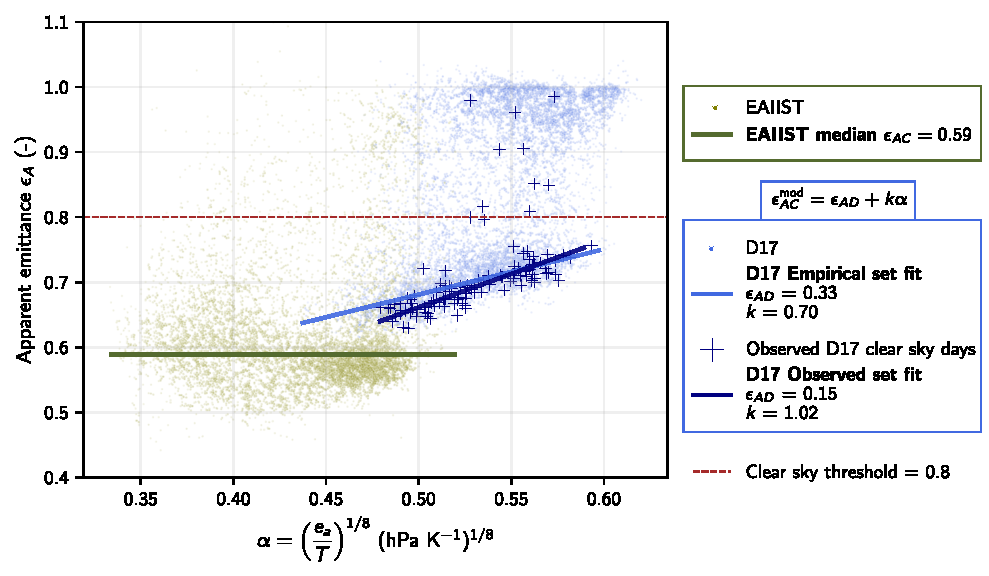
\includegraphics[width=16cm]{appemitt_scatter_def.pdf}
	\caption{\textbf{Apparent emissivity} | Test figure}
	\label{fig:appemit}
\end{figure}

	\section{Time series from Multiband and S-3 OLCI}

DDU very cool, EAIIST not so very cool, then...
	
	\section{Diagnostic of the results for EAIIST stations}
	
... then here we go

		\subsection{Multiband issues}
	
		\subsection{OLCI issues}
		
		\subsubsection{OLCI and Solalb: a comparison}
		
	Do not simply list the results, it can be boring
	If the comclusion from a result is very fast, just put it in the results

\setpartcolor{part4color}
\part{Discussion}
	
	\section{Considerations on the performance of the instruments}
	
	\section{Geoscientific interpretation of the time series}
Despite the imperfection of the results and the technical issues, some interesting interpretations about the signal recorded from both the \emph{in situ} equipment and the satellite can be drawn.

\setpartcolor{part5color}
\part{Conclusion}

\printbibliography[heading=bibintoc]
	
\end{document}
